\chapter{معرفی برنامه‌ی نمونه}
\label{chap:demoapp}

چارچوب تست برای ارزیابی، به یک
\lr{\gls{SUT}}
نیاز دارد؛ برنامه‌ای که به اندازه‌ی کافی پیچیده باشد تا توانایی چارچوب در تست «برنامه‌های پیچیده» را نشان دهد، اما همچنان در دامنه‌ی یک پروژه‌ی کارشناسی بماند. برای این منظور برنامه‌ی دسکتاپ «ردیاب سیگنال ایران» طراحی و پیاده‌سازی شد: سامانه‌ی پایش کیفیت سیگنال مخابراتی مبتنی بر
\lr{Qt C++}
و
\lr{SQLite}.
این فصل صرفاً معرفی‌کننده‌ی برنامه است؛ موضوع اصلی پایان‌نامه چارچوب تست است که در \autoref{chap:framework}
می‌آید.

\section{کارکرد برنامه}
برنامه از چهار بخش تشکیل شده است. نخست، دروازه‌ی ورود: کاربر باید با نام کاربری و گذرواژه وارد شود یا حساب جدید بسازد (شکل
\autoref{fig:signin})؛ حساب‌ها در همان پایگاه‌داده ذخیره می‌شوند و حساب مدیر امکان حذف کاربران را دارد. پس از ورود، پنجره‌ی اصلی با زبانه‌های «خانه»، «داده‌های شبکه»، «داشبورد» و «گزارش‌ها» در دسترس است.

\begin{figure}[H]
\centering
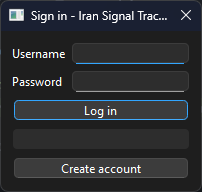
\includegraphics[width=0.5\linewidth]{fig_signin}
\caption{دروازه‌ی ورود برنامه‌ی نمونه}
\label{fig:signin}
\end{figure}

\section{داده‌های شبکه}
زبانه‌ی داده‌های شبکه (شکل
\autoref{fig:network})
هسته‌ی برنامه است: جدولی از نمونه‌های سیگنال با فیلترهای استان (با شهرهای آبشاری)، فناوری و اپراتور، جستجو، بازنشانی، خروجی
\lr{\gls{CSV}}
و نمودار ستونی میانگین کیفیت. برای مجموعه‌داده‌های بزرگ، جدول صفحه‌بندی می‌شود (اندازه‌های صفحه ۵۰ تا ۱۰۰۰) و نوار وضعیت همیشه اندازه‌ی کامل نتیجه را نشان می‌دهد.

\begin{figure}[H]
\centering
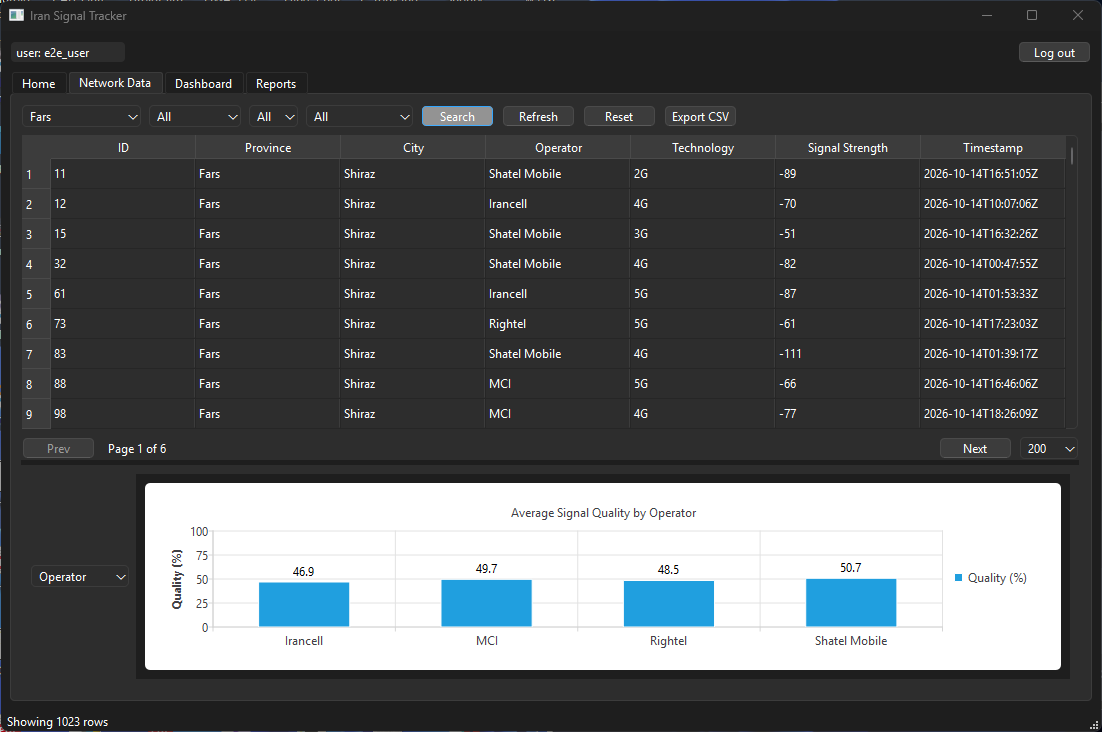
\includegraphics[width=\linewidth]{fig_network}
\caption{زبانه‌ی داده‌های شبکه؛ فیلتر استان فارس اعمال شده است}
\label{fig:network}
\end{figure}

\section{داشبورد و گزارش‌ها}
داشبورد (شکل
\autoref{fig:dashboard})
شاخص‌های کلیدی مانند میانگین کیفیت و تعداد نمونه‌ها، روند روزانه‌ی کیفیت، فهرست ضعیف‌ترین نمونه‌ها، نمودار دایره‌ای سهم اپراتورها و نمودار ستونی کیفیت بر حسب فناوری را نشان می‌دهد. هر دو نمودار جدید از فیلترهای همان زبانه تبعیت می‌کنند. زبانه‌ی گزارش‌ها (شکل
\autoref{fig:reports})
جدول خلاصه‌ی گروه‌بندی‌شده (بر اساس استان، اپراتور یا فناوری)، نمودار دایره‌ای سهم هر گروه، نمودار روند روزانه‌ی گروه انتخاب‌شده و خروجی
\lr{\gls{CSV}}
را ارائه می‌دهد.

\begin{figure}[H]
\centering
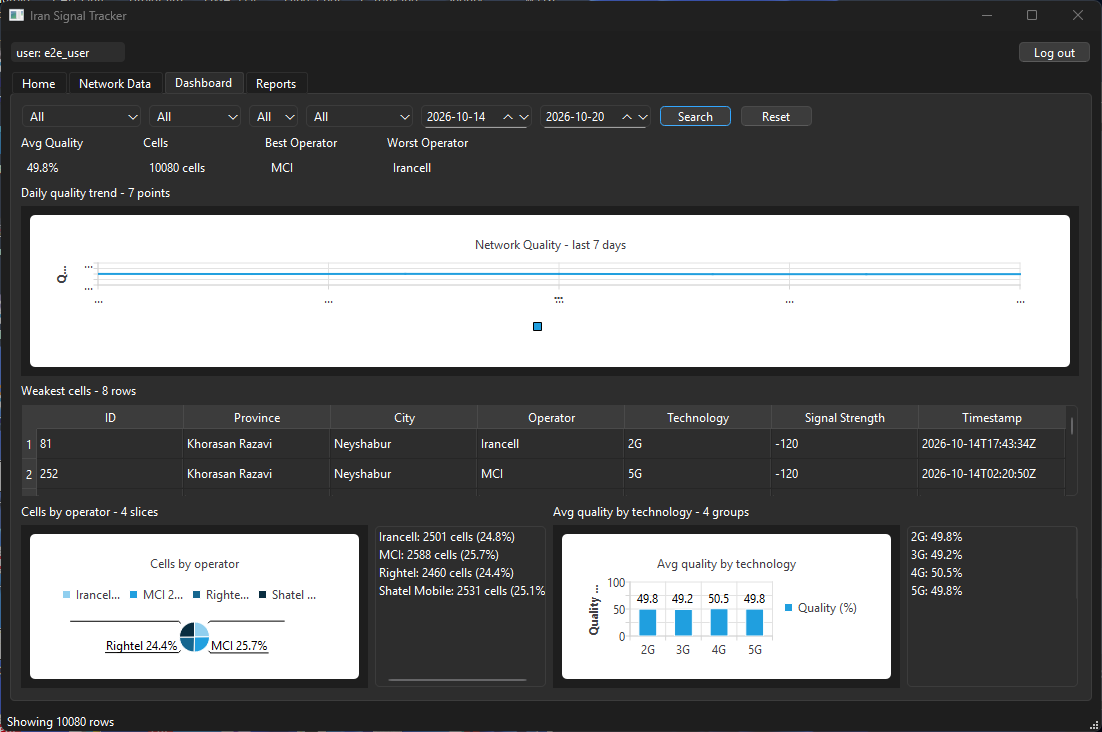
\includegraphics[width=\linewidth]{fig_dashboard}
\caption{داشبورد برنامه؛ نمودارهای دایره‌ای و ستونی سمت چپ و راست}
\label{fig:dashboard}
\end{figure}

\begin{figure}[H]
\centering
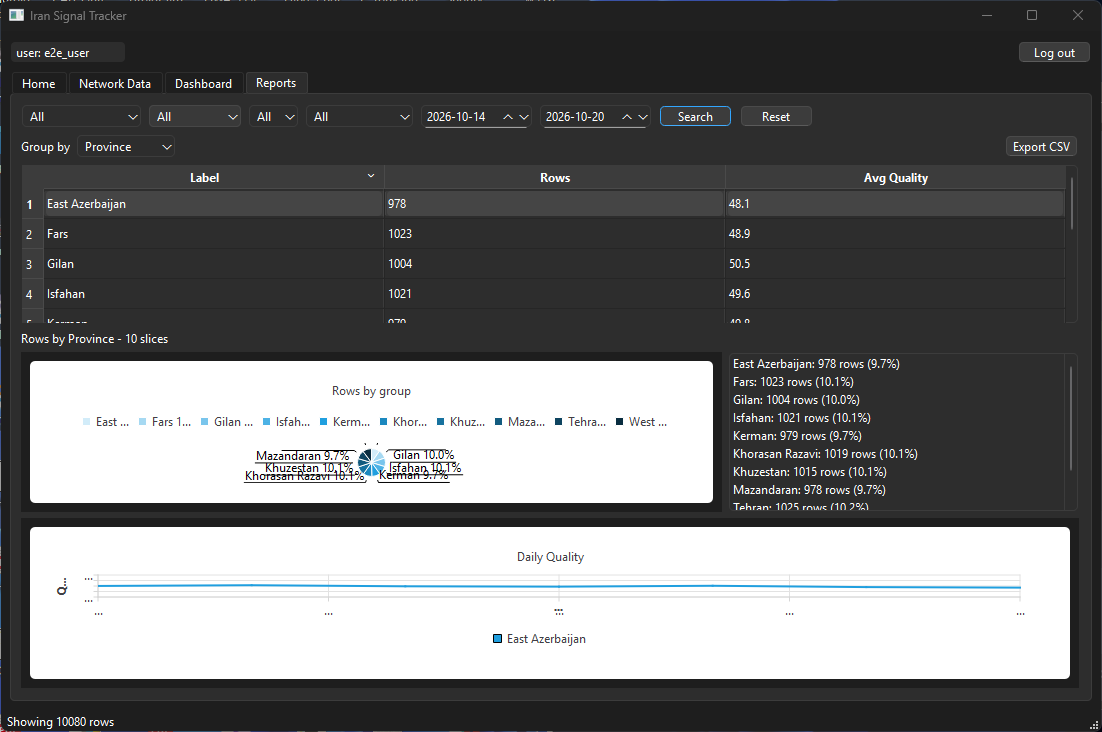
\includegraphics[width=\linewidth]{fig_reports}
\caption{زبانه‌ی گزارش‌ها؛ خلاصه‌ی گروه‌بندی‌شده، نمودار دایره‌ای و روند روزانه}
\label{fig:reports}
\end{figure}

\section{مجموعه‌داده}
داده‌ی برنامه یک مجموعه‌ی شبه‌واقعی از کیفیت سیگنال مخابراتی است: ۱۰٬۰۸۰ نمونه در بازه‌ی هفت روز (۱٬۴۴۰ نمونه در روز)، با تولید قطعی مبتنی بر بذر ثابت تا هر اجرا بازتولید‌پذیر باشد. داده‌ها شامل ده استان، شهرهای متناظر از نقشه‌ی دامنه‌ی برنامه، چهار اپراتور و چهار فناوری \lr{2G} تا \lr{5G} هستند. قدرت سیگنال هر نمونه به سنجه‌ی کیفیت ۰ تا ۱۰۰ درصد نگاشت می‌شود و همه‌ی نمودارها از این نگاشت مشترک تغذیه می‌کنند.

این برنامه آگاهانه ویژگی‌هایی را دارد که تست سرتاسری را دشوار می‌کند: جریان ورود با پنجره‌های متعدد، فیلترهای وابسته به هم، صفحه‌بندی، مجازی‌سازی جدول، نمودارهای گرافیکی که داده‌شان در درخت دسترس‌پذیری دیده نمی‌شود و دو نقش کاربری. همین دشواری‌ها معیار ارزیابی چارچوب در \autoref{chap:evaluation}
هستند.